\documentclass{article}
\usepackage[english]{babel}
\usepackage[a4paper,top=2cm,bottom=2cm,left=3cm,right=3cm,marginparwidth=1.75cm]{geometry}

% Packages
\usepackage{amsmath}
\usepackage{tikz}
\usepackage{caption}
\usepackage{algorithm}
\usepackage{algpseudocode}
%\usepackage{graphicx}
%\usepackage[colorlinks=true, allcolors=blue]{hyperref}

\tikzset{
  treenode/.style = {align=center, circle, black, inner sep=0pt, text centered,
    font=\sffamily, draw=black, text width=1.5em, very thick}
}

\title{Succinct Data Structure for Balanced Parentheses Sequences Representation}
\author{Fabrizio Brioni}

\begin{document}
\maketitle

\begin{abstract}
This document will describe a succinct structure to store and perform operations on balanced parentheses sequence. Initially the segment tree data structure will be described, followed by a description of a two-level organization (similar to the Jacobson rank structure) for storing information about balanced parentheses sequences and then an explanation of how to integrate the two structures to handle the operations \texttt{find\_close}, \texttt{find\_open}, \texttt{find\_enclose} efficiently and succinctly.
\end{abstract}

\section{Introduction}
A sequence $V$ of parentheses is balanced if in each prefix of $V$ the number of open parentheses is greater than or equal to the number of closed parentheses, and the total number of open parentheses in $V$ is equal to the number of closed parentheses. In a less formal way it can be defined as a sequence of parentheses from which a valid arithmetic operation can be obtained by adding some numbers and operations. Some useful operations on such sequences are the following:
    \begin{itemize}
    \item \texttt{find\_close(i)}: given an open parenthesis with index $i$, calculate the index of the corresponding closed parenthesis;
    \item \texttt{find\_open(i)}: given a closed parenthesis with index $i$, calculate the index of the corresponding open parenthesis;
    \item \texttt{find\_enclose(i)}: given a parenthesis with index $i$, calculate the positions $(x,y)$ of matching parentheses enclosing it. If there are multiple pairs with this property, select the innermost one, that is the one that does not contain other valid pairs (for a more formal definition read the \textbf{Notations}). 
    \end{itemize}
This document will show how, given a balanced parentheses sequence of length $2n$, perform such operations with a time complexity of $\mathcal{O}(\log{n})$ using $2n + o(n)$ bits of memory.

\section{Notations}
Let $v$ be a sequence of parentheses of length $2n$ numbered from $0$ to $2n-1$ and $v_i$ the parenthesis with index $i$. For convenience, assume a value of $v_i=1$ indicates an open parenthesis at position $i$ and a value of $v_i=0$ indicates a closed parenthesis at position of $i$. We define the excess of a position $i$ as:
    $$
    \text{excess}_v(i) = |\{j :\ j<i \land v_i=1\}|-|\{j :\ j\leq i \land v_i=0\}|
    $$
that is the difference between the number of open parentheses preceding $i$ (excluded) and the number of closed parentheses preceding $i$ (included).
It follows that a sequence of parentheses is balanced if and only if:
    \begin{align*}
    \text{excess}_v(i) &\geq 0 \qquad 0\leq i < 2n-1 \\
    \text{excess}_v(2n-1) &= 0
    \end{align*}
It also follows the definition of the operations of $\text{find\_close}, \text{find\_open}$ and $\text{find\_enclose}$:
    \begin{align*}
    \text{find\_close}_v(i) &= \min\{j :\ j>i \land \text{excess}_v(j)=\text{excess}_v(i)\} \\
    \text{find\_open}_v(i) &= \max\{j :\ j<i \land \text{excess}_v(j)=\text{excess}_v(i)\} \\
    \text{left\_enclose}_v(i) &= \max\{j :\ j<i \land \text{excess}_v(j)+1=\text{excess}_v(i)\} \\
    \text{right\_enclose}_v(i) &= \text{find\_close}_v(\text{left\_enclose}_v(i)) = \min\{j :\ j>i \land \text{excess}_v(j)+1=\text{excess}_v(i)\} \\
    \text{find\_enclose}_v(i) &= (\text{left\_enclose}_v(i),\text{right\_enclose}_v(i))
    \end{align*}
We will use $t^v$ to indicate a sequence of integers of length $2n$ such that:
    $$
    t^v_i=\text{excess}_v(i) \qquad 0\leq i < 2n-1
    $$
Finally we define a function $\texttt{find\_succ}(x,i,v)$ that given a sequence $x_0,x_1,\dots$ of integers and two integers $i$ and $v$ returns the index of the first element that follows $x_i$ and has value less or equal $v$:
    $$
    \text{find\_succ}(x,i,v)=\min\{j :\ j>i \land x_j\leq v\}
    $$
similarly we define a function $\texttt{find\_prev}(x,i,v)$ that returns the index of the last element that precedes $x_i$ and has value less than or equal to $v$
    $$
    \text{find\_prev}(x,i,v)=\max\{j :\ j<i \land x_j\leq v\}
    $$

\section{Segment Tree}
A Segment Tree for a sequence $x_0,x_1,\dots,x_{n-1}$ of length $n$ is a binary tree that has a root node containing information about the entire sequence (such as sum, maximum or minimum) and (if $n \neq 1$) having as left subtree a Segment Tree relative to the sequence $x_0,\dots,x_{\left\lfloor{\frac{n-1}{2}}\right\rfloor}$ and having as right subtree a SegmentTree relative to the sequence $x_{\left\lfloor{\frac{n-1}{2}}\right\rfloor+1},\dots,x_{n-1}$. Given a node $k$ of that tree, with $k.data$ we will indicate the information contained in that node (in our case we will always store the minimum element in the range of competence) and with $k.left$ and $k.right$ we will indicate the left and right child respectively.
    \begin{center}
        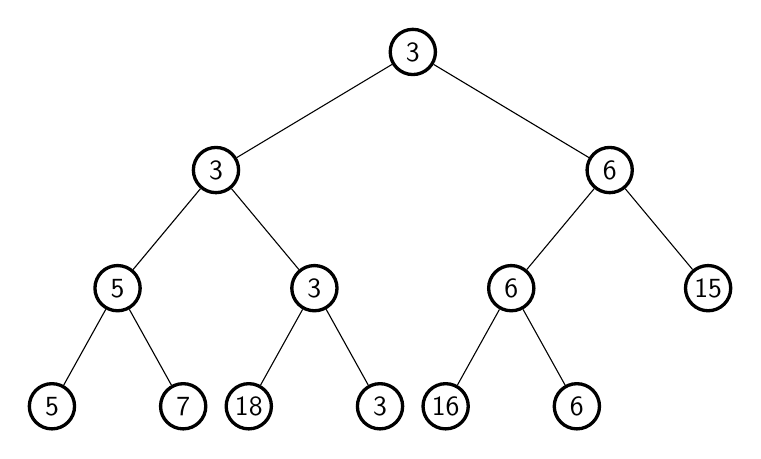
\begin{tikzpicture}[level/.style={sibling distance = 5cm/#1,
          level distance = 1.5cm}] 
        \node [treenode] {3}
            child{ 
                node [treenode] {3} 
                child{ 
                    node [treenode] {5} 
                	child{ 
                	    node [treenode] {5} 
                	}
        			child{
        			    node [treenode] {7}
        			}
                }
                child{ 
                    node [treenode] {3}
        			child{ 
        			    node [treenode] {18}
        			}
        			child{
        			    node [treenode] {3}
        			}
                }                            
            }
            child{ 
                node [treenode] {6}
                child{ 
                    node [treenode] {6} 
        			child{ 
        			    node [treenode] {16}
        			}
        			child{
        			    node [treenode] {6}
        			}
                }
                child{ 
                    node [treenode] {15}
                }
        	}
        ;
        \end{tikzpicture}
        \captionsetup{type=figure, width=.76\linewidth}
        \captionof{figure}{Segment tree for the sequence $5,7,18,3,16,6,15$. Each node contains the minimum value of the corresponding sequence.}
    \end{center}

\subsection{Construction}
The following procedure returns the Segment Tree root for the sequence $x$ of length $n=size(x)$:
    \begin{algorithmic}[1]
    \Procedure{Build}{$x$}
        \State $root\gets$\Call{Recursive\_build}{$x,0,size(x)-1$}
        \State \textbf{return} $root$
    \EndProcedure
    \State
    \Function{Recursive\_build}{$x,l,r$}
        \State $tmp\gets\text{new Segment Tree node}$
        \If{$l=r$}
            \State $tmp.data\gets x_l$
            \State $tmp.left\gets null$
            \State $tmp.right\gets null$
        \Else
            \State $tmp.left\gets$\Call{Recursive\_build}{$x,l,\left\lfloor{\frac{l+r}{2}}\right\rfloor$}
            \State $tmp.right\gets$\Call{Recursive\_build}{$x,\left\lfloor{\frac{l+r}{2}}\right\rfloor+1,r$}
            \State $tmp.data\gets\min\{tmp.left.data,tmp.right.data\}$
        \EndIf
        \State \textbf{return} $tmp$
    \EndFunction
    \end{algorithmic}
For a sequence of length $n$ the number of nodes created is:
    \begin{align*}
        f(n)=
        \begin{cases}
            1 \qquad &n=1 \\
            1+f(\left\lfloor{\frac{n}{2}}\right\rfloor)+f(\left\lceil{\frac{n}{2}}\right\rceil) \qquad &n>1
        \end{cases}
    \end{align*}
it follows that $f(n)=\mathcal{O}(n)$ and since the function \texttt{Recursive\_build} is called once for each node, the complexity of the construction procedure is $\mathcal{O}(n)$. Also assuming that each element of the sequence has a value between $0$ and $A$, the number of bits needed to contain the information of all nodes is $\mathcal{O}(n\log{A})$.

\subsection{find\_succ and find\_prev}
With this data structure it is possible to efficiently implement the function $\text{find\_succ}(x,i,v)$ after building the Segment Tree related to $x$ (whose root is \texttt{root}):
    \begin{algorithmic}[1]
    \Procedure{Find\_succ}{$root,x,i,v$}
        \State \textbf{return} \Call{Find\_succ\_recursive}{$root,i,v,0,size(x)-1$}
    \EndProcedure
    \State
    \Function{Find\_succ\_recursive}{$node,ind,val,l,r$}
        \If{$ind\geq r \lor node.data>val$}
            \State $res\gets\infty$
        \ElsIf{$l=r$}
            \State $res\gets l$
        \Else
            \State $res\gets$\Call{Find\_succ\_recursive}{$node.left,ind,val,l,\left\lfloor{\frac{l+r}{2}}\right\rfloor$}
            \If{$res\neq \infty$}
                \State $res\gets$\Call{Find\_succ\_recursive}{$node.right,ind,val,\left\lfloor{\frac{l+r}{2}}\right\rfloor+1,r$}
            \EndIf
        \EndIf
        \State \textbf{return} $res$
    \EndFunction
    \end{algorithmic}
The number of nodes visited and the complexity of this procedure is $\mathcal{O}(\log{n})$. In a similar way we can implement the procedure $\text{find\_prev}(x,i,v)$:
    \begin{algorithmic}[1]
    \Procedure{Find\_prev}{$root,x,i,v$}
        \State \textbf{return} \Call{Find\_prev\_recursive}{$root,i,v,0,size(x)-1$}
    \EndProcedure
    \State
    \Function{Find\_prev\_recursive}{$node,ind,val,l,r$}
        \If{$ind\leq l \lor node.data>val$}
            \State $res\gets -\infty$
        \ElsIf{$l=r$}
            \State $res\gets l$
        \Else
            \State $res\gets$\Call{Find\_prev\_recursive}{$node.right,ind,val,\left\lfloor{\frac{l+r}{2}}\right\rfloor+1,r$}
            \If{$res\neq -\infty$}
                \State $res\gets$\Call{Find\_prev\_recursive}{$node.left,ind,val,l,\left\lfloor{\frac{l+r}{2}}\right\rfloor$}
            \EndIf
        \EndIf
        \State \textbf{return} $res$
    \EndFunction
    \end{algorithmic}

\section{Two level organization of the information}
Given a sequence $v$ of balanced parentheses of length $2n$, divide it into \textit{super blocks} of size $\log^2{2n}$ (first level) and divide each super block into \textit{blocks} of size $\log{2n}$ (second level) and let $k=\log{2n}$.

\subsection{First Level}
The number of super blocks in this level is $\frac{2n}{k^2}$ (numbered from $0$ to $\frac{2n}{k^2}-1$), for each of them calculate the minimum excess present obtaining the sequence $S$:
    $$
    S_i = \min_{ik^2 \leq j < (i+1)k^2}\{t^v_j\} \qquad 0\leq i < \frac{2n}{k^2}
    $$
Build a Segment Tree for this sequence: since the elements of $t^v$ are between $0$ and $2n$ (because they are the excesses of a sequence of $2n$ parentheses) and the sequence $S$ has length $\frac{2n}{k^2}$, that Segment Tree will occupy $\mathcal{O}(\frac{2n}{k^2}\log{2n})=\mathcal{O}(\frac{2n}{\log{2n}})=o(n)$ bits.

Then calculate the sequence $T$ composed of the initial excess of each super block:
    $$
    T_i = t^v_{ik^2} \qquad 0\leq i < \frac{2n}{k^2}
    $$
if we store the sequence $T$ in an array the number of bits needed will also be $ \frac{2n}{k^2}\log{2n}=o(n)$, so the total number of bits used to store this first layer of information is $o(n)$.

\subsection{Second Level}
The number of blocks in this level is $\frac{2n}{k}$ (numbered from $0$ to $\frac{2n}{k}-1$), for each of them calculate the minimum excess present as a difference to the initial excess of its super block:
    $$
    B_i = \left(\min_{ik \leq j < (i+1)k}\{t^v_j\}\right)-T_{\left\lfloor{\frac{i}{k}}\right\rfloor} \qquad 0\leq i < \frac{2n}{k}
    $$
if we save the sequence $B$ in an array the number of bits needed is $\frac{2n}{k}\log{(2(\log{2n})^2)}=\frac{2n}{\log{2n}}\times$ $\times(2\log{\log{2n}}+\log{2})=o(n)$ because each element of $B$ will be between $-(\log{2n})^2$ and $(\log{2n})^2$.

Let's also calculate the sequence $A$ of the differences between the initial excess of each block and the initial excess of its super block:
    $$
    A_i = t^v_{ik}-T_{\left\lfloor{\frac{i}{k}}\right\rfloor} \qquad 0\leq i < \frac{2n}{k}
    $$
if we save the sequence $A$ in an array the number of bits needed is $\frac{2n}{k}\log{(2(\log{2n})^2)}=o(n)$, so in total the number of bits used to store this second layer of information is $o(n)$.

\section{find\_close and find\_open}
Once built the Segment Tree $S$ (whose root will be indicated with \texttt{root}) and calculated the values of $T$, $B$ and $A$ relative to the sequence of parentheses $v$ you can perform the operation \texttt{find\_close(i)} (assuming the parenthesis in position $i$ is open) as follows:
    \begin{enumerate}
        \item Calculate the excess $u = t^v_i = T_{\left\lfloor{\frac{i}{k^2}}\right\rfloor}+A_{\left\lfloor{\frac{i}{k}}\right\rfloor} + (t^v_i-t^v_{k\left(\left\lfloor{\frac{i}{k}}\right\rfloor\right)})= T_{\left\lfloor{\frac{i}{k^2}}\right\rfloor}+A_{\left\lfloor{\frac{i}{k}}\right\rfloor}+2\sum_{j=k(\left\lfloor{\frac{i}{k}}\right\rfloor)}^{i-1} v_j-(i-k(\left\lfloor{\frac{i}{k}}\right\rfloor))+(1-v_{k(\left\lfloor{\frac{i}{k}}\right\rfloor)})$. It can be calculated in $\mathcal{O}(\log{n})$ (the summation contains at most $\log{2n}$ addends);
        \item Check if the searched position belongs to the same block of the index $i$ by performing a linear scan of all parentheses following $i$ until the end of the block it belongs to ($v_{i+1},\dots,v_{k(\left\lfloor{\frac{i}{k}}\right\rfloor+1)-1}$): if there is an index $x$ such that the number of open and closed parentheses between $i$ and $x$ is equal then $x$ is the position searched for. During this process, there are at most $k=\log{2n}$ accesses to the sequence $v$;
        \item Otherwise check if the searched position belongs to the same super block of the index $i$ by scanning the values of $B$ related to blocks after $i$ until the end of the super block that $i$ belongs to ($B_{\left\lfloor{\frac{i}{k}}\right\rfloor+1},\dots,B_{k(\left\lfloor{\frac{i}{k^2}}\right\rfloor+1)-1}$): if there is an index $x$ such that $B_x+T_{\left \lfloor{\frac{i}{k^2}}\right\rfloor} \leq t^v_i$ then the searched position belongs to the block $x$ (and this block is in the same super block of the index $i$), in this case to find the exact position in the block is sufficient a scan of all the parentheses of that block ($v_{xk},v_{xk+1},\dots,v_{xk+k-1}$) until the first index $y$ such that $t^v_y=t^v_i$ (note how you can calculate the value of $t^v_y$ during the scan using the same formula of step $1$). During this process, there are at most $k=\log{2n}$ accesses to the sequence $B$ and at most $k=\log{2n}$ accesses to the sequence $v$;
        \item If the position was not found after the steps $2$ and $3$ means that the searched position is in another super block than the one where $i$ is, to find that super block just call the procedure \texttt{Find\_succ}$(B,\left\lfloor{\frac{i}{k^2}}\right\rfloor,t^v_i)$ that will return the index $x$ of the first super block that follows $i$ containing an excess less than or equal to $t^v_i$ (and since two consecutive values of $t^v$ differ by at most $1$, that super block will definitely contain an excess equal to $t^v_i$). At that point you have to search for the block where the searched position is located and then search for the exact position in a similar way as explained in step $3$: scan the values of $B$ relative to the blocks contained in the super block $x$ ($B_{xk},\dots,B_{xk+k-1}$) and if there is an index $y$ such that $B_y+T_x \leq t^v_i$ then the searched position is in the block $y$, finally to find the exact index you need to scan all the parentheses of that block ($v_{yk},\dots,v_{yk+k-1}$) until you find the first index $z$ such that $t^v_z=t^v_i$. During this process a call is made to the function \texttt{Find\_succ} (which has complexity $\mathcal{O}(\log{\frac{2n}{k^2}})=\mathcal{O}(\log{n})$) and there are at most $k=\log{2n}$ accesses to the sequence $B$ and at most $k=\log{2n}$ accesses to the sequence $v$;
    \end{enumerate}
In conclusion you can do the operation \texttt{find\_close} with complexity $\mathcal{O}(\log{n})$ using the sequence $v$ of parentheses that occupies $2n$ bits and other auxiliary structures (the Segment Tree related to the sequence $S$ and the sequences $T,B,A$) that occupy $o(n)$ bits. The following pseudocode shows the implementation of the whole procedure:
    \begin{algorithm}
    \caption{\texttt{Find\_close}}\label{findclose}
    \begin{algorithmic}[1]
    \Procedure{Find\_close}{$root,T,A,B,n,v,i$}\Comment{assume $v_i$ is an open parenthesis}
        \State $k\gets\log{2n}$
        \State $u\gets T_{\left\lfloor{\frac{i}{k^2}}\right\rfloor}+A_{\left\lfloor{\frac{i}{k}}\right\rfloor}-(i-k(\left\lfloor{\frac{i}{k}}\right\rfloor))$\Comment{step 1}
        \For{$j\gets k(\left\lfloor{\frac{i}{k}}\right\rfloor)\ \textbf{to}\ i-1$}
            \State $u\gets u+v_j$
        \EndFor
        \State $u\gets u+(1-v_{k(\left\lfloor{\frac{i}{k}}\right\rfloor)})$
        \State
        \State $tmp\gets 0$\Comment{step 2}
        \For{$x\gets i\ \textbf{to}\ k(\left\lfloor{\frac{i}{k}}\right\rfloor+1)-1$}
            \If{$v_x=1$}
                \State $tmp\gets tmp+1$
            \Else  
                \State $tmp\gets tmp-1$
            \EndIf
            \If{$tmp=0$}
                \State \textbf{return} $x$
            \EndIf
        \EndFor
        \State
        \For{$x\gets \left\lfloor{\frac{i}{k}}\right\rfloor+1\ \textbf{to}\ k(\left\lfloor{\frac{i}{k^2}}\right\rfloor+1)-1$}\Comment{step 3}
            \If{$B_x+T_{\left\lfloor{\frac{i}{k^2}}\right\rfloor} \leq u$}
                \State $currt\gets T_{\left\lfloor{\frac{i}{k^2}}\right\rfloor}+A_x$
                \For{$y\gets xk\ \textbf{to}\ xk+k-1$}
                    \If{$currt=u$}
                        \State \textbf{return} $y$
                    \EndIf
                    \If{$v_y=1$}
                        \State $currt\gets currt+1$
                    \EndIf
                    \If{$v_{y+1}=0$}
                        \State $currt\gets currt-1$
                    \EndIf
                \EndFor
    \algstore{alg1}            
    \end{algorithmic}
    \end{algorithm}
    \begin{algorithm}
    \begin{algorithmic}[1]
    \algrestore{alg1}
            \EndIf
        \EndFor
        \State
        \State $x\gets \Call{Find\_succ}{root,B,\left\lfloor{\frac{i}{k^2}}\right\rfloor,u}$ \Comment{step 4}
        \For{$y\gets xk\ \textbf{to}\ xk+k-1$}
            \If{$B_y+T_x \leq u$}
                \State $currt\gets T_x+A_y$
                \For{$z\gets yk\ \textbf{to}\ yk+k-1$}
                    \If{$currt=u$}
                        \State \textbf{return} $z$
                    \EndIf
                    \If{$v_z=1$}
                        \State $currt\gets currt+1$
                    \EndIf
                    \If{$v_{z+1}=0$}
                        \State $currt\gets currt-1$
                    \EndIf
                \EndFor
            \EndIf
        \EndFor
    \EndProcedure
    \end{algorithmic}
    \end{algorithm}
    
Symmetrically you can implement the operation \texttt{find\_open(i)}: just note that the operation \texttt{find\_open(i)} related to a sequence $v=v_0,\dots,v_{2n-1}$ is equivalent to a \texttt{find\_(2n-1-i)} related to the sequence $v_{2n-1},\dots,v_0$. Initially we check if the searched position is in the same block of $i$, otherwise we check if it is present in the same super block of $i$ and otherwise we search for the correct super block, the correct block within the super block and finally the exact position within the block:
    \begin{algorithm}[H]
    \caption{\texttt{Find\_open}}\label{findopen}
    \begin{algorithmic}[1]
    \Procedure{Find\_open}{$root,T,A,B,n,v,i$}\Comment{assume $v_i$ is a closed parenthesis}
        \State $k\gets\log{2n}$
        \State $u\gets T_{\left\lfloor{\frac{i}{k^2}}\right\rfloor}+A_{\left\lfloor{\frac{i}{k}}\right\rfloor}-(i-k(\left\lfloor{\frac{i}{k}}\right\rfloor)+1)$\Comment{step 1}
        \For{$j\gets k(\left\lfloor{\frac{i}{k}}\right\rfloor)\ \textbf{to}\ i-1$}
            \State $u\gets u+v_j$
        \EndFor
        \State $u\gets u+(1-v_{k(\left\lfloor{\frac{i}{k}}\right\rfloor)})$
        \State
        \State $tmp\gets 0$\Comment{step 2}
        \For{$x\gets i\ \textbf{down to}\ k\left\lfloor{\frac{i}{k}}\right\rfloor$}
            \If{$v_x=1$}
                \State $tmp\gets tmp+1$
            \Else  
                \State $tmp\gets tmp-1$
            \EndIf
            \If{$tmp=0$}
                \State \textbf{return} $x$
            \EndIf
        \EndFor
        \State
        \For{$x\gets \left\lfloor{\frac{i}{k}}\right\rfloor-1\ \textbf{down to}\ k(\left\lfloor{\frac{i}{k^2}}\right\rfloor)$}\Comment{step 3}
            \If{$B_x+T_{\left\lfloor{\frac{i}{k^2}}\right\rfloor} \leq u$}
                \State $currt\gets T_{\left\lfloor{\frac{i}{k^2}}\right\rfloor}+A_{x+1}$
                \For{$y\gets xk+k-1\ \textbf{down to}\ xk$}
                    \If{$v_{y+1}=0$}
                        \State $currt\gets currt+1$
                    \EndIf
                    \If{$v_y=1$}
    \algstore{alg1}            
    \end{algorithmic}
    \end{algorithm}
    \begin{algorithm}[ht]
    \begin{algorithmic}[1]
    \algrestore{alg1}
                        \State $currt\gets currt-1$
                    \EndIf
                    \If{$currt=u$}
                        \State \textbf{return} $y$
                    \EndIf
                \EndFor
            \EndIf
        \EndFor
        \State
        \State $x\gets \Call{Find\_prev}{root,B,\left\lfloor{\frac{i}{k^2}}\right\rfloor,u}$ \Comment{step 4}
        \For{$y\gets xk+k-1\ \textbf{down to}\ xk$}
            \If{$B_y+T_x \leq u$}
                \If{$y<xk+k-1$}
                    \State $currt\gets T_x+A_{y+1}$
                \Else
                    \State $currt\gets T_{x+1}$
                \EndIf
                \For{$z\gets yk+k-1\ \textbf{down to}\ yk$}
                    \If{$v_{z+1}=0$}
                        \State $currt\gets currt+1$
                    \EndIf
                    \If{$v_z=1$}
                        \State $currt\gets currt-1$
                    \EndIf
                    \If{$currt=u$}
                        \State \textbf{return} $z$
                    \EndIf
                \EndFor
            \EndIf
        \EndFor
    \EndProcedure
    \end{algorithmic}
    \end{algorithm}
\section{Find\_enclose}
The operation \texttt{left\_enclose(i)} is analogous to \texttt{find\_open(i)} with the only difference that the excess searched is not $t^v_i$ but $t^v_i-1$ (and there is no solution if $t^v_i=0$):
    \begin{algorithm}[H]
    \caption{\texttt{Left\_enclose}}\label{leftenclose}
    \begin{algorithmic}[1]
    \Procedure{Left\_enclose}{$root,T,A,B,n,v,i$}
        \State $k\gets\log{2n}$
        \State $u\gets T_{\left\lfloor{\frac{i}{k^2}}\right\rfloor}+A_{\left\lfloor{\frac{i}{k}}\right\rfloor}-(i-k(\left\lfloor{\frac{i}{k}}\right\rfloor))$\Comment{step 1}
        \For{$j\gets k(\left\lfloor{\frac{i}{k}}\right\rfloor)\ \textbf{to}\ i-1$}
            \State $u\gets u+v_j$
        \EndFor
        \State $u\gets u+(1-v_{k(\left\lfloor{\frac{i}{k}}\right\rfloor)})$
        \If{$v_i=0$}
            \State $u\gets u-1$
        \EndIf
        \State $u\gets u-1$\Comment{the excess searched now is $t^v_i-1$}
        \If{u=-1}
            \State \textbf{return} $-1$ \Comment{not found}
        \EndIf
        \State
        \State $tmp\gets u+1$\Comment{step 2}
        \For{$x\gets i\ \textbf{down to}\ k\left\lfloor{\frac{i}{k}}\right\rfloor$}
            \If{$tmp=u$}
                \State \textbf{return} $x$
            \EndIf
    \algstore{alg1}            
    \end{algorithmic}
    \end{algorithm}
    \begin{algorithm}[ht]
    \begin{algorithmic}[1]
    \algrestore{alg1}
            \If{$v_x=0$}
                \State $tmp\gets tmp+1$
            \EndIf
            \If{$v_{x-1}=1$}
                \State $tmp\gets tmp-1$
            \EndIf
        \EndFor
        \For{$x\gets \left\lfloor{\frac{i}{k}}\right\rfloor-1\ \textbf{down to}\ k(\left\lfloor{\frac{i}{k^2}}\right\rfloor)$}\Comment{step 3}
            \If{$B_x+T_{\left\lfloor{\frac{i}{k^2}}\right\rfloor} \leq u$}
                \State $currt\gets T_{\left\lfloor{\frac{i}{k^2}}\right\rfloor}+A_{x+1}$
                \For{$y\gets xk+k-1\ \textbf{down to}\ xk$}
                    \If{$v_{y+1}=0$}
                        \State $currt\gets currt+1$
                    \EndIf
                    \If{$v_y=1$}
                        \State $currt\gets currt-1$
                    \EndIf
                    \If{$currt=u$}
                        \State \textbf{return} $y$
                    \EndIf
                \EndFor
            \EndIf
        \EndFor
        \State
        \State $x\gets \Call{Find\_prev}{root,B,\left\lfloor{\frac{i}{k^2}}\right\rfloor,u}$ \Comment{step 4}
        \For{$y\gets xk+k-1\ \textbf{down to}\ xk$}
            \If{$B_y+T_x \leq u$}
                \If{$y<xk+k-1$}
                    \State $currt\gets T_x+A_{y+1}$
                \Else
                    \State $currt\gets T_{x+1}$
                \EndIf
                \For{$z\gets yk+k-1\ \textbf{down to}\ yk$}
                    \If{$v_{z+1}=0$}
                        \State $currt\gets currt+1$
                    \EndIf
                    \If{$v_z=1$}
                        \State $currt\gets currt-1$
                    \EndIf
                    \If{$currt=u$}
                        \State \textbf{return} $z$
                    \EndIf
                \EndFor
            \EndIf
        \EndFor
    \EndProcedure
    \end{algorithmic}
    \end{algorithm}
And therefore the operation \texttt{find\_enclose} is just a call to \texttt{left\_enclose} and to \texttt{find\_close}:
    \begin{algorithm}[H]
    \caption{\texttt{Find\_enclose}}\label{findenclose}
    \begin{algorithmic}[1]
    \Procedure{Find\_enclose}{$root,T,A,B,n,v,i$}
    \State $x\gets$ \Call{Left\_enclose}{$root,T,A,B,n,v,i$}
    \If{$x=-1$}
        \State \textbf{return} $(-1,-1)$ \Comment{no solution}
    \Else
        \State \textbf{return} $(x,$\Call{Find\_close}{$x$}$)$
    \EndIf
    \EndProcedure
    \end{algorithmic}
    \end{algorithm}
\section{Conclusions}
It has been shown how to perform the operations \texttt{find\_close}, \texttt{find\_open} and \texttt{find\_enclose} with $\mathcal{O}(\log{n})$ complexity using $2n+o(n)$ bits. The initial construction of all the necessary structures has complexity $\mathcal{O}(n)$.
\end{document}